\documentclass[10pt, landscape]{article}
\usepackage[scaled=0.92]{helvet}
\usepackage{calc}
\usepackage{multicol}
\usepackage{ifthen}
\usepackage[a4paper,margin=3mm,landscape]{geometry}
\usepackage{amsmath,amsthm,amsfonts,amssymb}
\usepackage{color,graphicx,overpic}
\usepackage{hyperref}
\usepackage{newtxtext} 
\usepackage{enumitem}
\usepackage{amssymb}
\usepackage[table]{xcolor}
\usepackage{vwcol}
\usepackage{tikz}
\usetikzlibrary{arrows.meta}
\usetikzlibrary{calc}
\usepackage{mathtools}
\usepackage{nicematrix}
%For pictures / figures
\usepackage{color,graphicx,overpic}
\graphicspath{ {./images/} }
% for relations
\usepackage{cancel}
\usepackage{ mathrsfs }
\graphicspath{ {./images/} }
\setlist{nosep}


\pdfinfo{
  /Title (GEA1000-Final.pdf)
  /Creator (TeX)
  /Producer (pdfTeX 1.40.0)
  /Author (Seamus)
  /Subject (Example)
  /Keywords (pdflatex, latex,pdftex,tex)}

% Turn off header and footer
\pagestyle{empty}

\newenvironment{tightcenter}{%
  \setlength\topsep{0pt}
  \setlength\parskip{0pt}
  \begin{center}
}{%
  \end{center}
}

% redefine section commands to use less space
\makeatletter
\renewcommand{\section}{\@startsection{section}{1}{0mm}%
                                {-1ex plus -.5ex minus -.2ex}%
                                {0.5ex plus .2ex}%x
                                {\normalfont\large\bfseries}}
\renewcommand{\subsection}{\@startsection{subsection}{2}{0mm}%
                                {-1explus -.5ex minus -.2ex}%
                                {0.5ex plus .2ex}%
                                {\normalfont\normalsize\bfseries}}
\renewcommand{\subsubsection}{\@startsection{subsubsection}{3}{0mm}%
                                {-1ex plus -.5ex minus -.2ex}%
                                {1ex plus .2ex}%
                                {\normalfont\small\bfseries}}%
\renewcommand{\familydefault}{\sfdefault}
\renewcommand\rmdefault{\sfdefault}
% makes nested numbering (e.g. 1.1.1, 1.1.2, etc)
\renewcommand{\labelenumii}{\theenumii}
\renewcommand{\theenumii}{\theenumi.\arabic{enumii}.}
\renewcommand\labelitemii{•}
%  for logical not operator
\renewcommand{\lnot}{\mathord{\sim}}
\renewcommand{\bf}[1]{\textbf{#1}}
\newcommand{\abs}[1]{\vert #1 \vert}
\newcommand{\Mod}[1]{\ \mathrm{mod}\ #1}

\makeatother
\definecolor{myblue}{cmyk}{1,.72,0,.38}
\everymath\expandafter{\the\everymath \color{myblue}}
% Define BibTeX command
\def\BibTeX{{\rm B\kern-.05em{\sc i\kern-.025em b}\kern-.08em
    T\kern-.1667em\lower.7ex\hbox{E}\kern-.125emX}}
\let\iff\leftrightarrow
\let\Iff\Leftrightarrow
\let\then\rightarrow
\let\Then\Rightarrow

% Don't print section numbers
\setcounter{secnumdepth}{0}

\setlength{\parindent}{0pt}
\setlength{\parskip}{0pt plus 0.5ex}
%% this changes all items (enumerate and itemize)
\setlength{\leftmargini}{0.5cm}
\setlength{\leftmarginii}{0.5cm}
\setlist[itemize,1]{leftmargin=2mm,labelindent=1mm,labelsep=1mm}
\setlist[itemize,2]{leftmargin=4mm,labelindent=1mm,labelsep=1mm}

%My Environments
\newtheorem{example}[section]{Example}
% -----------------------------------------------------------------------

\begin{document}
\raggedright
\footnotesize
\begin{multicols}{4}


% multicol parameters
% These lengths are set only within the two main columns
\setlength{\columnseprule}{0.25pt}
\setlength{\premulticols}{1pt}
\setlength{\postmulticols}{1pt}
\setlength{\multicolsep}{1pt}
\setlength{\columnsep}{2pt}

\begin{center}
    \fbox{%
        \parbox{0.8\linewidth}{\centering \textcolor{black}{
            {\Large\textbf{GEA1000 Final}}
            \\ \normalsize{AY24/25 sem 2}}
            \\ {\footnotesize \textcolor{myblue}{github.com/mendax1234}} 
        }%
    }
\end{center}
\section{Getting Data}
\begin{enumerate}
    \item \textbf{Census}: A method of data collection or attempts to reach \textbf{everyone} in the \textbf{population}.
    \item \textbf{Bias}
    \begin{itemize}
        \item \textbf{Selection Bias}: Due to the \textbf{researcher}’s biased selection of units.
        \item \textbf{Non-response Bias}: Arises from \textbf{participants}’ non-participation or non-disclosure. e.g., sending out 2000 surveys, receiving only 500 responses.
    \end{itemize}
    \item \textbf{Probability Sampling}
    \begin{itemize}
        \item \textbf{Simple Random Sampling (SRS)}: Use a random generator to select each sampling unit. Any sample size $n$ must be \textbf{equally likely to be chosen}.
        \begin{itemize}
            \item \textbf{Advantages}: \textbf{No selection bias}. Larger sample size \textbf{reduces random errors}. 
            \item \textbf{Shortcoming}: Subject to \textbf{non-response} bias. Have to know the whole number of sampling units in the \textbf{sampling frame}.
        \end{itemize}
        \item \textbf{Systematic Sampling}: 
        \begin{itemize}
            \item \textbf{Sampling Example}:
            \begin{itemize}
                \item The population has $p$ sampling units in total
                \item We decide our sample to have $n$ units. We select \textbf{one unit} from every $k=\frac{p}{n}$ units;
                \item From 1 to $k$, select a number \textbf{at random}, say $r$
                \item With this, the sample will consist : $r, r+k, r+2k, \cdots,r+(n-1)$
            \end{itemize}
            \item \textbf{Advantage}: No need to know the whole sampling units in the \textbf{sampling frame}.
            \item \textbf{Shortcoming}: If the \textbf{sampling frame} is \textbf{not random}, the sample \textbf{may not be representative}.
        \end{itemize}
        \item \textbf{Stratified Sampling}:
        \begin{itemize}
            \item \textbf{Sampling Example}
            \begin{itemize}
                \item The sampling frame is divided into groups called \textbf{strata}. Each \textbf{stratum} is \textbf{shares similar characteristics} but the size \textbf{may be different}.
                \item SRS is then applied to each stratum to generate the whole sample.
            \end{itemize}
        \item \textbf{Shortcoming}: Hard to form such stratum.
        \end{itemize}
        \item \textbf{Cluster Sampling}:
        \begin{itemize}
            \item \textbf{Sampling Example}
            \begin{itemize}
                \item Divide the sampling frame into \textbf{clusters}, where \textbf{clusters} doesn't have any requirements for its inner sampling units, thus ensuring the \textbf{inner diversity}
                \item Use SRS to select \textbf{a fixed number of clusters}.
                \item All the sampling units from the selected clusters are then included in the overall sample.
            \end{itemize}
            \item \textbf{Tips}
            \begin{itemize}
                \item Clusters can be formed by grouping students' \textbf{name}.
            \end{itemize}
        \end{itemize}
        \item \textbf{Tips}
        \begin{itemize}
            \item In probability sampling, every sampling unit must have a \textbf{non-zero} chance to be selected.
        \end{itemize}
    \end{itemize}
    \item \textbf{Non-probability Sampling}
    \begin{itemize}
        \item \textbf{Convenience Sampling}: A \textbf{researcher }chooses the sampling units \textbf{by convenience}.
        \item \textbf{Volunteer Sampling}: The sampling units \textbf{volunteer} themselves into a sample, a.k.a \textbf{self-selected sampling}.
    \end{itemize}
    \item \textbf{Mean $\bar{x}$}: It is just \textbf{average}.
    \item \textbf{Median}: Sort the data first, then find the middle value. If total number is \textbf{even}, find the \textbf{average of the middle two} values.
    \item \textbf{Standard Deviation $s_x$}: It is computed using, $\sqrt{\frac{(x_1-\bar{x})^2+(x_2-\bar{x})^2+\cdots+(x_n-\bar{x})^2}{n-1}}$. Share the \textbf{same unit} as the \textbf{numerical variable} $x$. In histogram, the standard deviation reverses the intuitive.
    \item \textbf{Variance} = $s_x^2$ \\
    \begin{tabular}{|c|c|c|c|}
        \hline
        Operation & Mean & Median & Std Dev \\ \hline
        Add $c$ & $+$ $c$ & $+$ $c$ & No change \\ \hline
        Multiply by $c$ & $\times$ $c$ & $\times$ $c$ & $\times$ $|c|$ \\ \hline
    \end{tabular}
    \item \textbf{IQR}: IQR = $Q_3-Q_1$, to find $Q_3$ (75\% percentile) and $Q_1$ (25\% percentile), we can use
    \begin{itemize}
        \item \textbf{Find the median} of the total $n$ data points.
        \item \textbf{Divide the data into upper half and lower half} according to the median
        \begin{itemize}
            \item If $n$ is \textbf{even}, just divide normally
            \item If $n$ is \textbf{odd}, \textbf{exclude} the median from the \textbf{upper half}
        \end{itemize}
        \item \textbf{Find} $Q_1$ and $Q_3$
        \begin{itemize}
            \item $Q_1$ is the median of the \textbf{lower half}.
            \item $Q_3$ is the median of the \textbf{upper half}.
        \end{itemize}
    \end{itemize}
    \item \textbf{Types of variables}
    \begin{itemize}
        \item \textbf{Categorical Nominal Variable}: No intrinsic ordering. (e.g., ``yes/no'')
    \end{itemize}
    \item \textbf{Coefficient of variation} = $\frac{s_x}{\bar{x}}$, \textbf{no unit}
    \item \textbf{Generalisability}:
    \begin{itemize}
        \item The \textbf{sample frame} must be \textbf{greater than} the \textbf{population of interest}.
    \end{itemize}
    \item \textbf{Study Designs}
    \begin{itemize}
        \item \textbf{Experimental Studies}: \textbf{Manipulate} the independent variable, e.g. \textbf{researchers} assign them \textbf{treatment} or \textbf{placebo}, to see the effect of the dependent variable. 
        \begin{itemize}
            \item \textbf{Treatment Group}: Those who receives the ``treatment''
            \item \textbf{Control Group}: Those who \textbf{does not receive} the ``treatment'', or use the \textbf{existing treatment} given that we already know the effect of \textbf{no treatment}.
            \item \textbf{Placebo}: A \textbf{placebo} is a substance with \textbf{no actual effect} but is made to \textbf{look like the treatment}.
            \item \textbf{Can} provide \textbf{cause-and-effect relationship} if it has features of \textbf{randomized assignment} and \textbf{blinding} (preferably double blinding).
        \end{itemize}
        \item \textbf{Observational Study}: \textbf{Observes} individuals and measures the variables of interest, usually \textbf{without any direct/deliberate manipulation of the variables} by the researchers.
        \begin{itemize}
            \item We still use terms like \textbf{treatment} and \textbf{control groups}.
            \item For \textbf{observational studies}, subjects assign \textbf{themselves} into either the treatment or control group.
            \item \textbf{Observational studies cannot} provide cause-and-effect relationship.
            \item \textbf{No selection bias} in \textbf{observational studies}.
        \end{itemize}
        \item \textbf{Random Assignment}: Uses chance (or probability) to \textbf{allocate objects into treatment and control groups}.
        \begin{itemize}
            \item \textbf{Property 1}: If the number of subjects is large, by the law of probability, the subjects in the treatment and control groups will tend to be \textbf{similar in all aspects} (like \textbf{have similar characteristics}).
            \item \textbf{Property 2}: When performing random assignment, the size of \textbf{treatment group} and \textbf{control group} does not need to be \textbf{the same}.
        \end{itemize}
        \item \textbf{Blinding}
        \begin{itemize}
            \item \textbf{Double-blinding} doesn't ensure the \textbf{generalisability}.
        \end{itemize}
    \end{itemize}
\end{enumerate}

\section{Categorical Data Analysis}
\begin{enumerate}
    \item \textbf{Rate}: It is calculated as the ratio of the number of observations in a \textbf{given category} (a.k.a \textbf{target}) to the \textbf{total} number of observations (a.k.a \textbf{population}).
    \begin{itemize}
        \item \textbf{Tips}: Regarding rate problem, always find your \textbf{target} and \textbf{population}. Then $\text{rate}=\text{target}\div \text{population}$
    \end{itemize}
    \item \textbf{2x2 contingency table}: \textbf{Dependent Variables} at \textbf{columns}, \textbf{Independent variables} at \textbf{rows}. For example, \textbf{treatment} is independent variable, \textbf{outcome} is the dependent variable.
    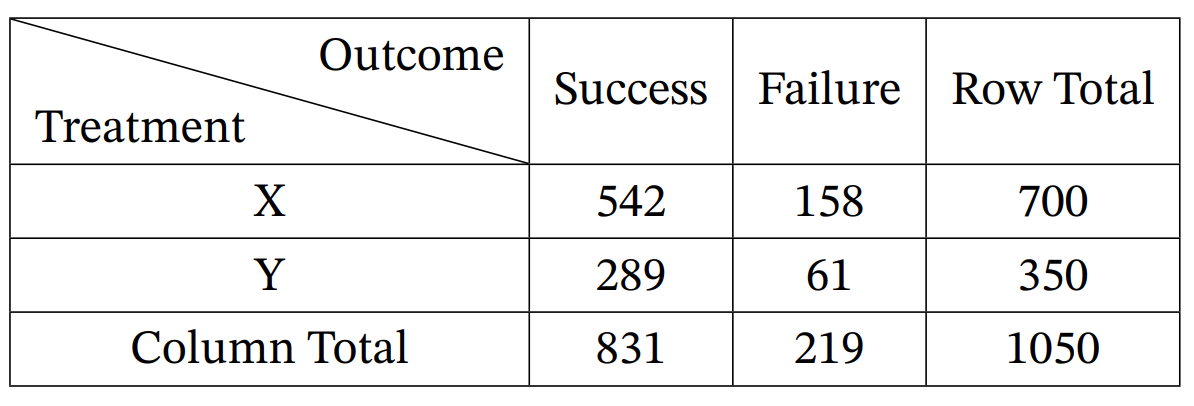
\includegraphics[width=1\linewidth]{images/1.png}
    \item \textbf{Marginal rate}: rate(A), \textbf{A} is the \textbf{target}, the \textbf{population} is the total by default.
    \item \textbf{Conditional rate}: rate($A\mid B$), our \textbf{target} will be the number of A under the condition B, our \textbf{population} will be the total number which satisfies the condition B.
    \item \textbf{Joint Rate}: $\text{rate}(A\cap B)$ our \textbf{target} will be the \textbf{intersection/and}, the \textbf{population} will be the whole population by default.
    \item \textbf{Association}: Describes a relationship between two \textbf{categorical variables}. Association $\neq$ causation.
    \begin{itemize}
        \item \textbf{Positive association}: rate($A \mid B$) $>$ rate($A \mid NB$). Meaning: the presence of A \textbf{when B is present} is \textbf{stronger} compared to when B is absent.
        \item \textbf{Negative association}: rate($A \mid B$) $<$ rate($A \mid NB$). Meaning: the presence of A \textbf{when B is present} is \textbf{weaker} compared to when B is absent. \\
        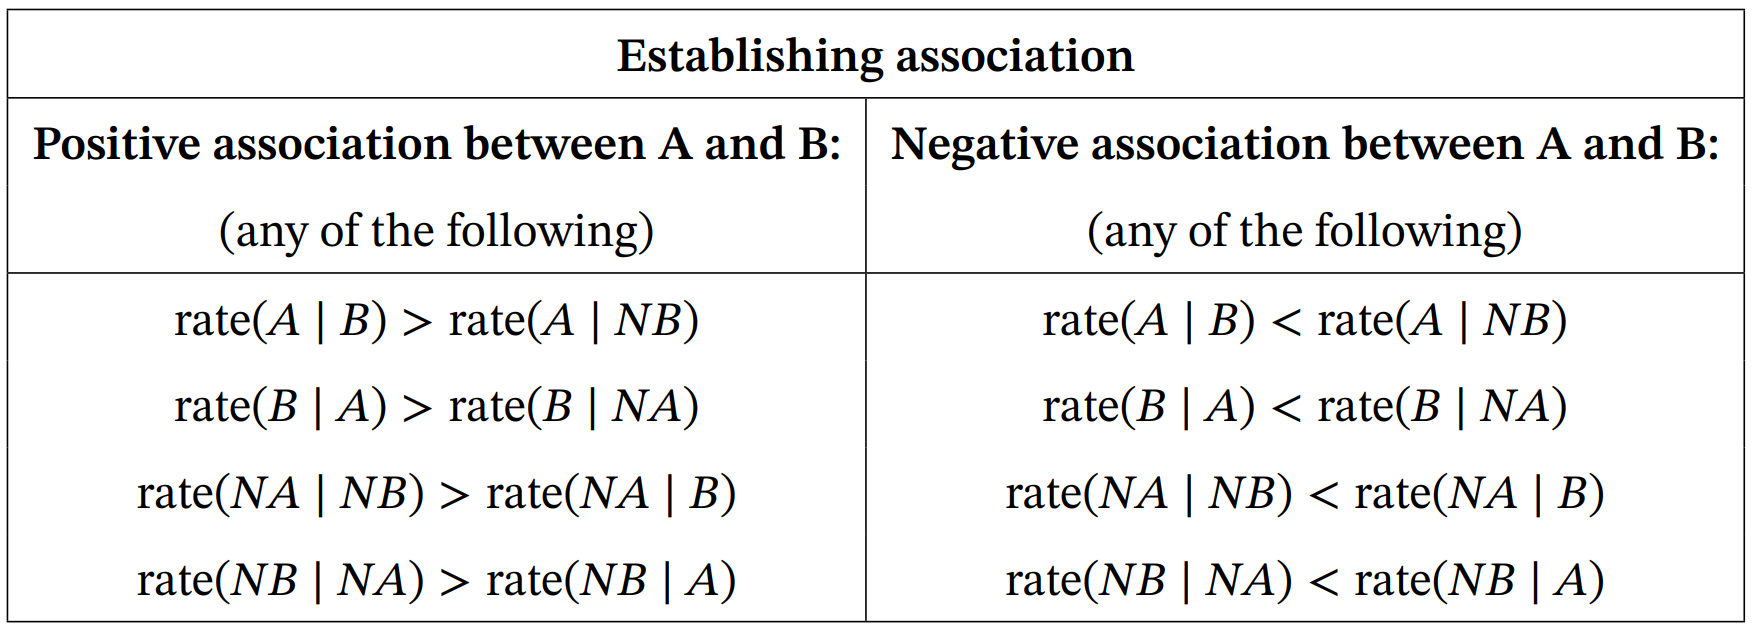
\includegraphics[width=1\linewidth]{images/2.png}
        \item \textbf{Tips}: Always find what \textbf{A} is and what \textbf{B} is.
    \end{itemize}
    \item \textbf{Two rules on rates}
    \begin{itemize}
        \item \textbf{Symmetric Rule}
            \begin{itemize}
                \item \textbf{Part 1}: $\text{rate}(A \mid B) > \text{rate}(A \mid NB) \Leftrightarrow \text{rate}(B \mid A) > \text{rate}(B \mid NA)$
                \item \textbf{Part 2}: $\text{rate}(A \mid B) < \text{rate}(A \mid NB) \Leftrightarrow \text{rate}(B \mid A) < \text{rate}(B \mid NA)$
                \item \textbf{Part 3}: $\text{rate}(A \mid B) = \text{rate}(A \mid NB) \Leftrightarrow \text{rate}(B \mid A) = \text{rate}(B \mid NA)$
            \end{itemize}
        \item \textbf{Basic Rule on Rates}: The overall $\text{rate}(A)$ will always lie between $\text{rate}(A \mid B)$ and $\text{rate}(A \mid NB)$
            \begin{itemize}
                \item \textbf{Consequence 1}: The closer $\text{rate}(B)$ is to 100\%, the closer $\text{rate}(A)$ is to $\text{rate}(A \mid B)$
                \item \textbf{Consequence 2}: If $\text{rate}(B)=50\%$, then $\text{rate}(A)=\frac{1}{2}[\text{rate}(A \mid B) + \text{rate}(A \mid NB)]$
                \item \textbf{Consequence 3}: If $\text{rate}(A \mid B)=\text{rate}(A \mid NB)$, then $\text{rate}(A) = \text{rate}(A \mid B) = \text{rate}(A \mid NB)$
                \item \textbf{Tips}: The bounds for the interval will change to whatever is smaller and bigger.
            \end{itemize}
    \end{itemize}
    \item \textbf{Simpson's Paradox}: If we divide the whole population into several subgroups, the trend that appears in \textbf{more than half of the subgroups} of data may \textbf{disappears or reverses} when the subgroups are combined, this is called \textbf{Simpson's Paradox}.
    \begin{itemize}
        \item The appearance of \textbf{simpson's paradox} implies the variable we use to slice is a \textbf{confounder}.
    \end{itemize}
    \item \textbf{Confounder}: A third variable that is \textbf{associated} with \textbf{both the independent and dependent variables}.
    \begin{itemize}
        \item The appearance of a \textbf{confounder} does not necessarily imply a \textbf{simpson's paradox}.
        \item Remove \textbf{one of the associations} is enough to remove the confounding variable.
    \end{itemize}
    \item \textbf{Tips}
    \begin{itemize}
        \item When building examples for questions regarding \textbf{median or mean}, be very careful! Use exhaustive thinking!
        \item $\text{rate(A}\mid\text{B)}$ is \textbf{not equal to} $\text{rate(B}\mid\text{A)}$!
        \item See words like \textbf{can}, build an example to prove!
    \end{itemize}
\end{enumerate}

\section{Dealing with Numerical Data}
\subsection{Univarite EDA}
\begin{enumerate}
    \item \textbf{Skewness}: Used only in \textbf{unimodal distribution} \\
    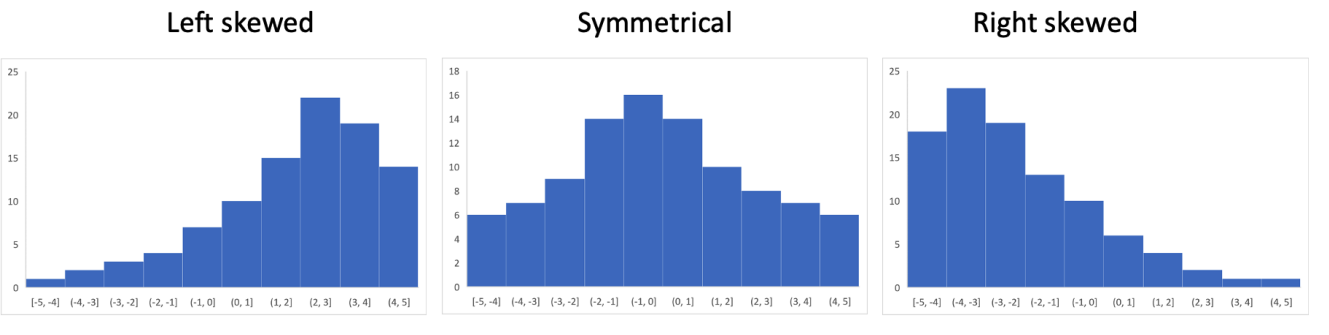
\includegraphics[width=1\linewidth]{images/3.png} \\
    And its central tendency is as follows \\
    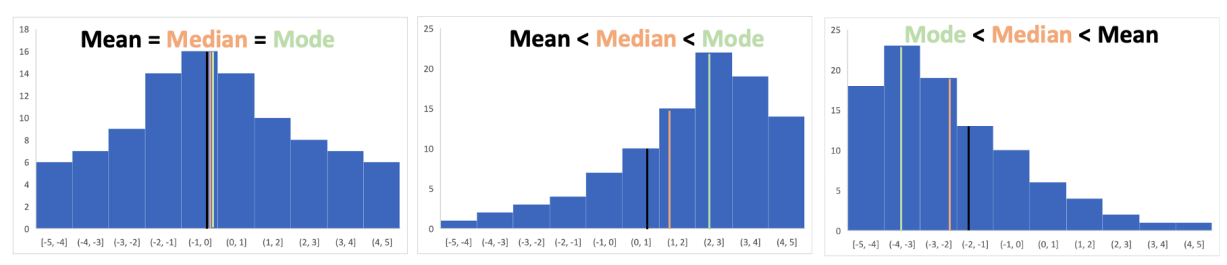
\includegraphics[width=1\linewidth]{images/4.png}
    \item \textbf{Range} = the largest data point - the smallest data point
    \item \textbf{Outlier}: If the value is either \textbf{greater than} $Q_3+1.5\times\text{IQR}$ or \textbf{less than} $Q_1-1.5\times\text{IQR}$ (Equal is \textbf{not include}! a.k.a, the range is \textbf{open}, not \textbf{bounded})
    \item \textbf{Bar Chart} \\
    \centerline{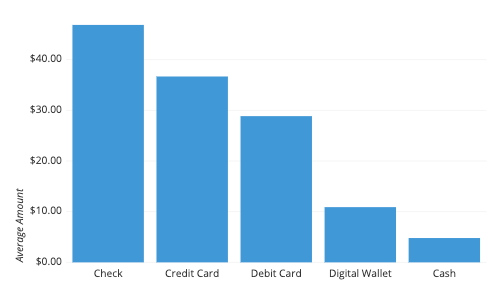
\includegraphics[width=0.5\linewidth]{images/8.png}}
    \begin{itemize}
        \item Used to display data for \textbf{categorical} variables (\textbf{not numerical variables})
        \item Typically have gaps between each bar
        \item The order of bars can be \textbf{rearranged freely}.
    \end{itemize}
    \item \textbf{Histogram}: \\
    \centerline{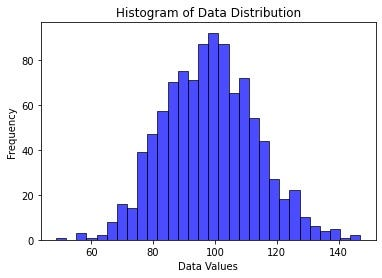
\includegraphics[width=0.5\linewidth]{images/7.png}}
    \begin{itemize}
        \item The width of each rectangle is called \textbf{bin width}.
        \item The number of \textbf{data points} we have in a \textbf{data set} is better shown in a \textbf{histogram} than in a \textbf{boxplot}.
    \end{itemize}
    \item \textbf{Boxplot}: \\
    \centerline{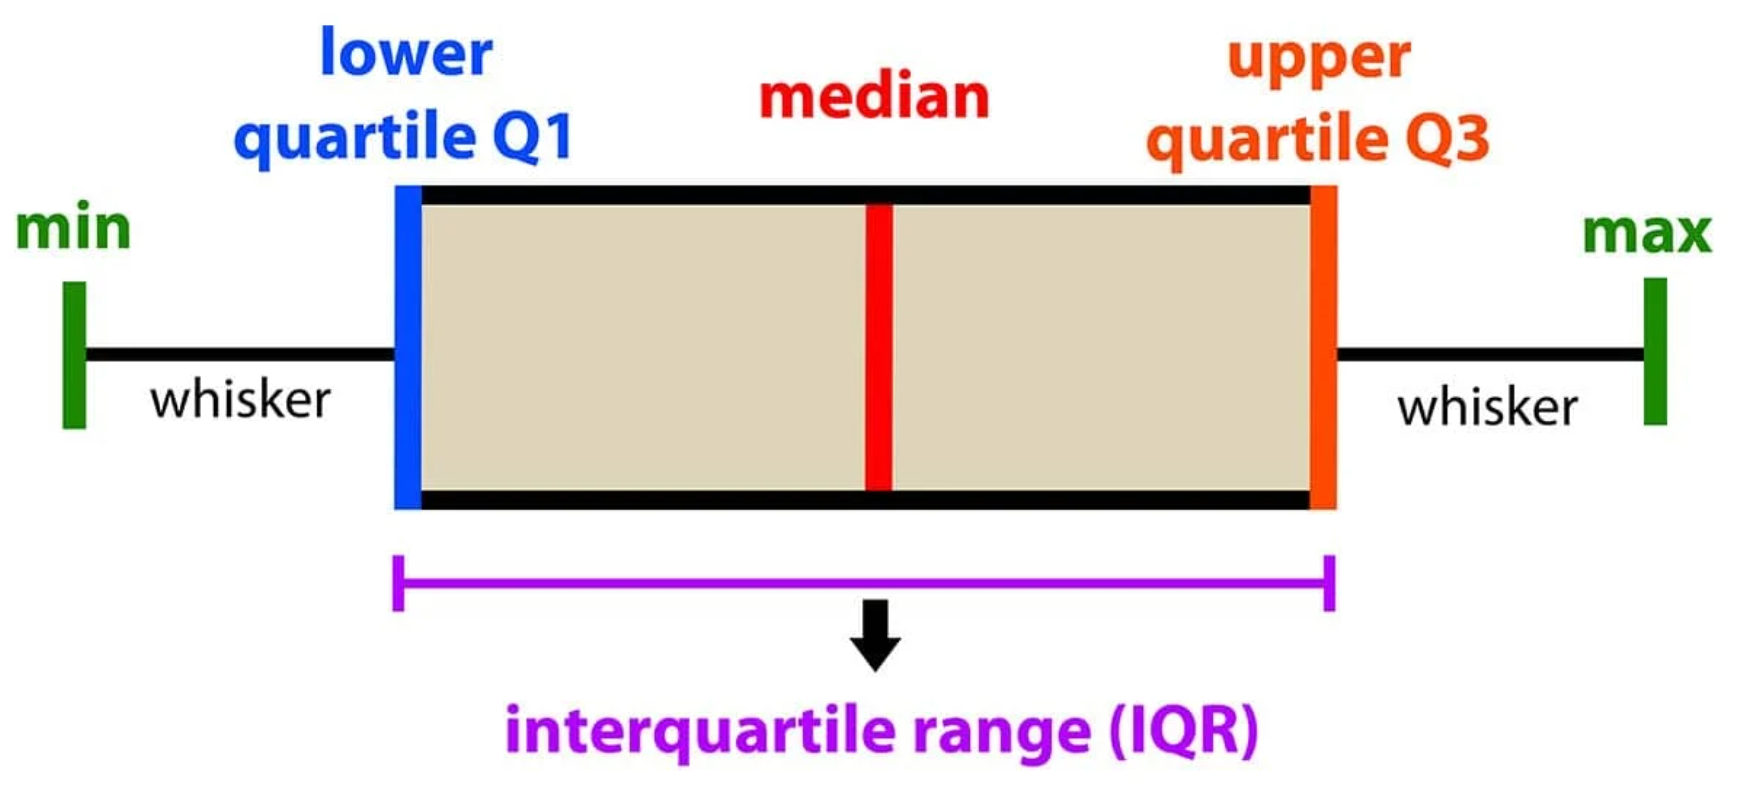
\includegraphics[width=0.8\linewidth]{images/6.png}}
    \begin{itemize}
        \item Sometimes the $\times$ near the \textbf{median} line is used to indicate the \textbf{mean}.
        \item \textbf{Outliers} are shown as \textbf{dots}, so the number of dots indicates how many outliers there are. Thus, \textbf{boxplots} are better at identifying outliers than \textbf{histograms}.
        \item \textbf{Identical boxplots} \textbf{do not imply} the same number of data points or the same standard deviation.
    \end{itemize}
    \item \textbf{Tips}
    \begin{itemize}
        \item When constructing the counterexample, the value in a data set can be \textbf{negative} unless restrictions are specified elsewhere.
        \item In \textbf{scatter plot}, an \textbf{outlier} is a data point that deviates significantly from the \textbf{overall pattern} (the cluster of points) or \textbf{trend of the other points} (the regression line of points)
    \end{itemize}
\end{enumerate}
\subsection{Bivariate EDA}
\begin{enumerate}
    \item \textbf{Direction}: describes the \textbf{relationship} between two variables. Can be \textbf{positive, negative or neither}.
    \item \textbf{Form}: Describe the overall \textbf{shape} of a scatter plot. It is classified into \textbf{linear} and \textbf{non-linear} (which may include quadratic or exponential patterns)
    \item \textbf{Correlation Coefficient}: A measure of \textbf{linear} association between two numerical variables. Always between -1 and 1. The \textbf{sign} of \(r\) reveals the direction, while the \textbf{magnitude} (how close \(r\) is to 1 or \(-1\)) indicates the \textbf{strength} of the association.
    \begin{itemize}
        \item \textbf{Three properties related to $r$}: $r$ is \textbf{not} affected by 1)\textbf{interchanging} the $x$ and $y$ variables, 2)\textbf{adding} a number to \textbf{all} values of a variable and 3)\textbf{multiplying} a \textbf{positive} number to \textbf{all} values of a variable.
        \item \textbf{How removing outliers will affect $r$} \\
        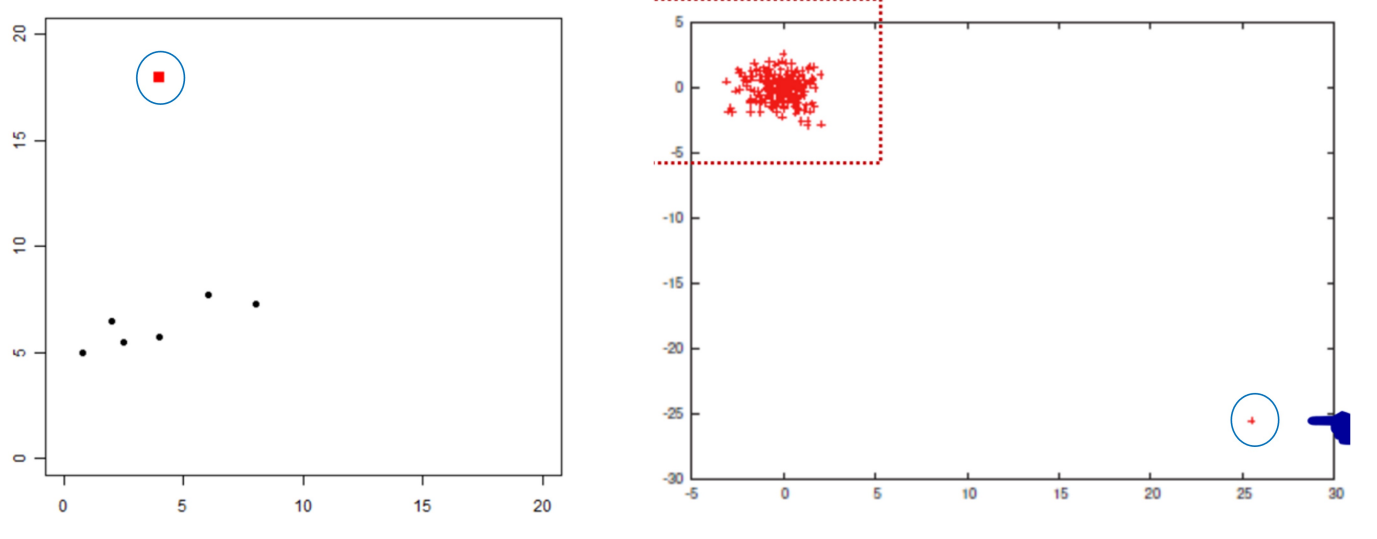
\includegraphics[width=1\linewidth]{images/9.png}
        \begin{itemize}
            \item In the Left figure, removing outlier will \textbf{increase} the \textbf{strength}
            \item In the right figure, removing outlier will \textbf{decrease} the \textbf{strength}. e.g., $r$ decreases from 0.75 to 0.01.
            \item Removing the outlier may also \textbf{not change} the $r$.
        \end{itemize}
        \item $r$ has \textbf{sign}, thus \textbf{not having the same} change as \textbf{strength}, be careful!
    \end{itemize}
    \item \textbf{Ecological Fallacy}: Use \textbf{aggregate level} correlation to conclude \textbf{individual level correlation}.
    \item \textbf{Atomistic Fallacy}: The reverse of Ecological Fallacy.
    \item \textbf{Linear Regression}:
    \begin{itemize}
        \item The linear regression line \textbf{always} pass through the average point $(\bar x, \bar y)$.
        \item Make prediction only \textbf{within the range of independent variable}.
        \item Removing the outlier may \textbf{increase, decrease or not change} the \textbf{slope} of the linear regression line.
    \end{itemize}
    \item \textbf{Tips}
    \begin{itemize}
        \item \textbf{Association} is \textbf{not causation}.
        \item The correlation coefficient $r$ does not tell anything about \textbf{non-linear} relationship. While $r$ for a non-linear relationship can be small, its relationship may be actually \textbf{strong}.
        \item Correlation coefficient $r$ has the \textbf{same sign} with the \textbf{slope of the linear regression line}.
    \end{itemize}
\end{enumerate}

\section{Statistical Inference}
\subsection{Probability}
\begin{enumerate}
    \item \textbf{Basic Terms}:
    \begin{itemize}
        \item \textbf{Sample space}: The collection of \textbf{all possible outcomes} of a probability experiment. e.g. [HH, TT, HT, TH]
        \item \textbf{Event}: A \textbf{sub-collection} of the sample space is called an \textbf{event}. (Think it as \textbf{subset})
        \item \textbf{Outcome}: It is exactly the event of \textbf{one element} in the sample space.
    \end{itemize}
    \item \textbf{Conditional Probability}: $P(E\mid F)=\frac{P(E\cap F)}{P(F)}$, which means the probability of E to happen \textbf{given that} F happens.
    \item \textbf{Prosecutor's fallacy}: The mistake of confusing $P(A\mid B)$ as $P(B \mid A)$
    \item \textbf{Independent Event}: We say two events $A$ and $B$ are \textbf{independent} if and only if $P(A\cap B)=P(A)\times P(B)$
    \item \textbf{Mutually Exclusive Event}: Two events \textbf{cannot} happen together, which means $P(E\cap F)=0$. $E$ and $F$ are mutually exclusive if and only if $P(E\cup F)=P(E)+P(F)$
    \item \textbf{Conditional Independency}: We say that two events $A$ and $B$ are \textbf{conditionally independent} given an event $C$ if $P(A\cap B \mid C)=P(A\mid C)\times P(B\mid C)$
    \item \textbf{Law of total probability}: If $E, F,G$ are events from the same sample space $S$ such that 1) $E$ and $F$ are mutually exclusive, and 2)$E\cup F=S$, then $P(G)=P(G\cap E)+P(G\cap F)=P(G\mid E)\times P(E)+P(G\mid F)\times P(F)$
    \item \textbf{Conjunction Fallacy}: You think that the probability of two things happening together is \textbf{greater} than one thing happens. But \textbf{it is not true}!
    \item \textbf{Base rate fallacy}: The mistake that only \textbf{sensitivity and specificity} are given, but \textbf{base rate} is ignored.
    \begin{itemize}
        \item \textbf{Sensitivity}: This is same as \textbf{true positive rate}. e.g. $P(\text{Test positive} \mid \text{Individual is infected})$
        \item \textbf{Specificity}: This is same as \textbf{true negative rate}. e.g. $P(\text{Test negative} \mid \text{Individual is not infected})$
        \item \textbf{Base rate}: e.g. The infection rate $P(\text{Individual is infected})$
        \item Regarding this kind of question, always \textbf{build a 2x2 contingency table}. Always start from the \textbf{conditional base rate} or the \textbf{base rate}. Then use \textbf{sensitivity} and \textbf{specificity}.
    \end{itemize}
    \item \textbf{Random Variable} \\
    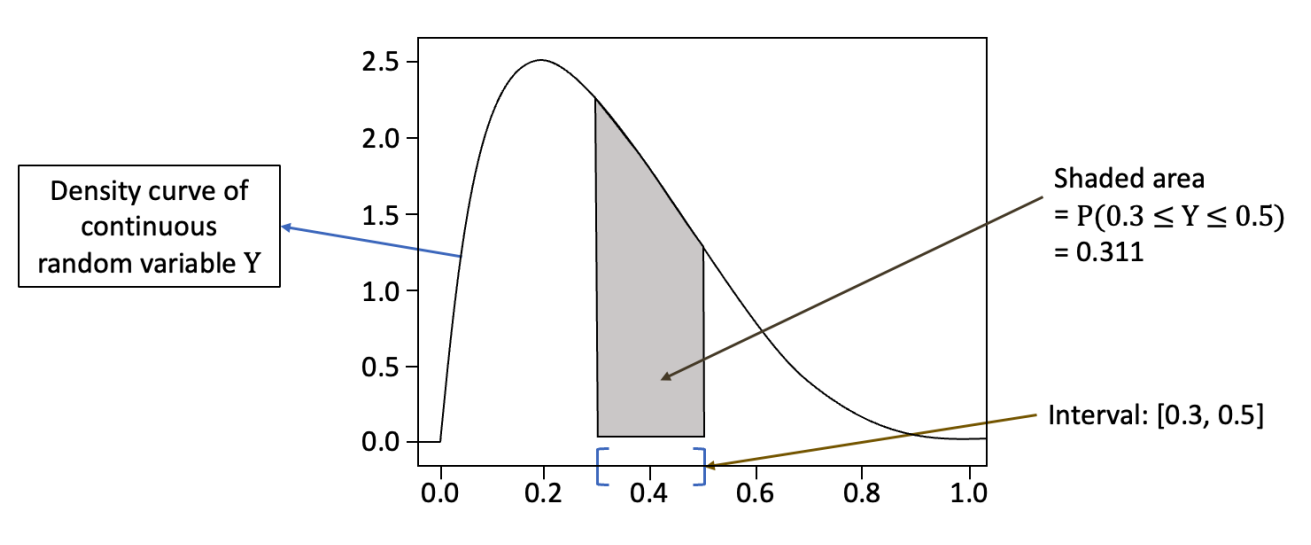
\includegraphics[width=1\linewidth]{images/10.png} \\
    x-axis is the possible value for the random variable $Y$, y-axis is the \textbf{probability density}. This graphs means $P(0.3\leq Y\leq 0.5)=0.311$
\end{enumerate}
\subsection{Confidence Interval}
\begin{enumerate}
    \item \textbf{For population proportion}
    \begin{itemize}
        \item \textbf{Formula}: $p^*\pm z^*\times\sqrt{\frac{p^*(1-p^*)}{n}}$, where $p^*=\text{sample proportion}, z^*=\text{``z-value'' from standard normal distribution}, n=\text{sample size}$
        \item \textbf{$z^*$ value}: 90\% CI, $z^*=1.645$, 95\%CI, $z^*=1.96$. More confident, $z^*$ bigger.
    \end{itemize}
    \item \textbf{For population mean}
    \begin{itemize}
        \item \textbf{Formula}: $\bar{x}\pm t^*\times \frac{s}{\sqrt{n}}$, where $\bar{x}=\text{sample mean}, t^*=\text{``t-value'' from t-distribution}, s=\text{sample standard deviation}, n=\text{sample size}$
        \item \textbf{$t^*$ value}: More confident, $t^*$ bigger.
    \end{itemize}
    \item \textbf{Margin of error}: The term after $\pm$ in the formula.
    \item \textbf{Interpretation}: If \textbf{many simple random samples} of the same size are taken, and a \textbf{confidence level} is constructed for each of them, then about \textbf{95\% of the CI} constructed would contain the \textbf{population parameter}. But every CI will contain its corresponding \textbf{sample population parameter}.
    \item \textbf{Properties of CI}
    \begin{itemize}
        \item The \textbf{larger the sample size} $n$, the \textbf{smaller the random error} (a.k.a margin error).
        \item The \textbf{higher the confidence level} at which the CI is constructed (a.k.a the larger the $z^*$ or $t^*$), \textbf{the wider the CI}.
    \end{itemize}
    \item \textbf{Tips}
    \begin{itemize}
        \item Given a CI with the \textbf{same sample}, always calculate the \textbf{sample population parameter} and the \textbf{margin of error}.
        \item CI is a way to \textbf{quantify} the random of error.
        \item CI constructed from \textbf{sample} is \textbf{likely} to include the population parameter. But if CI is constructed from \textbf{population}, it confirms to contain the \textbf{population parameter}.
    \end{itemize}
\end{enumerate}
\subsection{Hypothesis Testing}
\begin{enumerate}
    \item \textbf{Definition}: A \textbf{hypothesis test} is a statistical inference method used to decide if the data from a random or even more extreme is \textbf{sufficient} to support a particular hypothesis about a population.
    \item \textbf{Two cases}:
    \begin{itemize}
        \item a population parameter is $x$ (denoted as Case 1)
        \item in the population, 2 categorical variables A and B are associated with each other. (denoted as Case 2)
    \end{itemize}
    \item \textbf{Null hypothesis}
    \begin{itemize}
       \item In case 1, it says population parameter $p$ equals to a specific value.
       \item In case 2, it means there is \textbf{no association} (Independence) between the two categorical variables.
    \end{itemize}
    \item \textbf{Alternative hypothesis}
    \begin{itemize}
        \item In case 1, it says population parameter $p \neq$ a specific value.
        \item In case 2, it means there is \textbf{an association} (Dependence) between the two categorical variables.
    \end{itemize}
    \item \textbf{Five steps of hypothesis testing}
    \begin{itemize}
        \item Identify the question and state \textbf{the null hypothesis} and \textbf{alternative\textit{ hypothesis}}.
        \item Set the \textbf{significance level} of our test. It is often set at 5\%, can be 1\% and 10\% also.
        \item Using our sample, we find the relevant sample statistic. This means calculating the population parameter we want but using the \textbf{sample data}.
        \item With the sample statistic and the hypothesis, we can calculate the $p$-value.
        \item Make a conclusion of the hypothesis test.
        \begin{itemize}
            \item If the p-value is $\leq$ the significance level (e.g., 0.05), you \textbf{reject the null hypothesis} and say there is evidence for the alternative hypothesis.
            \item Otherwise, you \textbf{fail to reject the null hypothesis}, we don’t have enough evidence to support the alternative. (You don’t “accept” the null.)
        \end{itemize}
    \end{itemize}
    \item \textbf{The meaning of p-value}: The probability of obtaining a result \textbf{as extreme} or \textbf{more extreme} than our observation (the value calculated using the sample data) \textbf{in the direction of alternative hypothesis} (This means following the direction!), assuming \textbf{the null hypothesis is true}.
    \item \textbf{Tips}
    \begin{itemize}
        \item For example, if your suspect is biased \textbf{against} heads, your \textbf{alternative hypothesis} should be $P(\text{Heads})<0.5$
        \item \textbf{Steps to find other observations need to be considered when calculating p-value}
        \begin{itemize}
            \item Know the direction of your \textbf{alternative hypothesis}
            \item We need the observations \textbf{starting from the initial observation} and \textbf{follow the direction} in the above step. Just follow.
            \item \textbf{Decimal points}: the digits after the \textbf{.} e.g. 2 decimal points, 3.14
            \item \textbf{Significant points}: the number of digits starting from first non-zero. e.g., 2 significant points, 0.0045
        \end{itemize}
    \end{itemize}
\end{enumerate}

\end{multicols}

\end{document}